\chapter{Transizione da IPv4 a IPv6}

\section{Principi Generali e Obiettivi}
L'esaurimento dello spazio di indirizzamento di IPv4 è il motivo principale che ha spinto l'adozione di IPv6. Tuttavia, non è mai stata stabilita una data ufficiale ("switch-off") oltre la quale IPv4 smetterà improvvisamente di funzionare a livello globale. Di conseguenza, è inevitabile una lunga fase transitoria --- che dura ormai da decenni --- in cui entrambi i protocolli devono coesistere e operare simultaneamente.

Per garantire che questa transizione avvenga senza disservizi, sono stati definiti tre requisiti ideali:
\begin{itemize}
\item \textbf{Incrementale (Incremental):} La transizione deve poter avvenire gradualmente nel tempo. I dispositivi e le reti devono poter adottare IPv6 progressivamente, mantenendo il supporto a IPv4 finché necessario.
\item \textbf{Continua (Seamless):} Il passaggio non deve causare interruzioni di servizio. Le applicazioni e la connettività di base devono continuare a funzionare regolarmente.
\item \textbf{Trasparente (Smooth):} L'utente finale e l'host non devono accorgersi se i loro pacchetti stanno attraversando una rete IPv4, una rete IPv6, o se stanno subendo traduzioni intermedie. L'esperienza di rete deve risultare invariata.
\end{itemize}

Per raggiungere questi obiettivi, sono state sviluppate tre principali macro-categorie di meccanismi tecnologici:
\begin{enumerate}
\item \textbf{Dual-stack approach:} I dispositivi implementano contemporaneamente entrambi gli stack protocollari (IPv4 e IPv6). Sono in grado di generare, ricevere e instradare pacchetti per entrambe le versioni del protocollo a seconda della necessità.
\item \textbf{Address mapping:} Algoritmi e meccanismi per mappare indirizzi IPv4 in IPv6 e viceversa. Passare da 32 bit (IPv4) a 128 bit (IPv6) è semplice (tipicamente si aggiungono dei prefissi all'indirizzo IPv4), ma l'operazione inversa è molto complessa e richiede approcci specifici, poiché non è possibile comprimere 128 bit in 32 senza perdere informazioni.
\item \textbf{Tunneling e Translation:}
\begin{itemize}
\item Il \textit{Tunneling} consiste nell'incapsulare un pacchetto di un protocollo all'interno del payload di un altro (es. IPv6 dentro IPv4). Viene utilizzato quando due isole di una stessa famiglia di protocolli devono comunicare attraverso una rete nativa dell'altra famiglia.
\item La \textit{Translation} (Traduzione) prevede invece l'intervento di un router intermedio che modifica letteralmente l'header del pacchetto, convertendo i campi e gli indirizzi sorgente e destinazione da una versione all'altra.
\end{itemize}
\end{enumerate}

\section{Fasi di Adozione e Stato Attuale}
La transizione verso una rete puramente IPv6 è un percorso a tappe. Storicamente, possiamo suddividere l'evoluzione in quattro scenari (o "step") principali.


\begin{enumerate}
\item \textbf{Reti IPv6 isolate (Isolated IPv6 networks):} È lo scenario iniziale (anni '90/2000). La quasi totalità di Internet è IPv4. Le prime "isole" di host IPv6 (obbligatoriamente Dual-stack) comunicano tra loro incapsulando il traffico IPv6 all'interno di tunnel IPv4 per attraversare la rete geografica.

\begin{figure}[H]
\centering
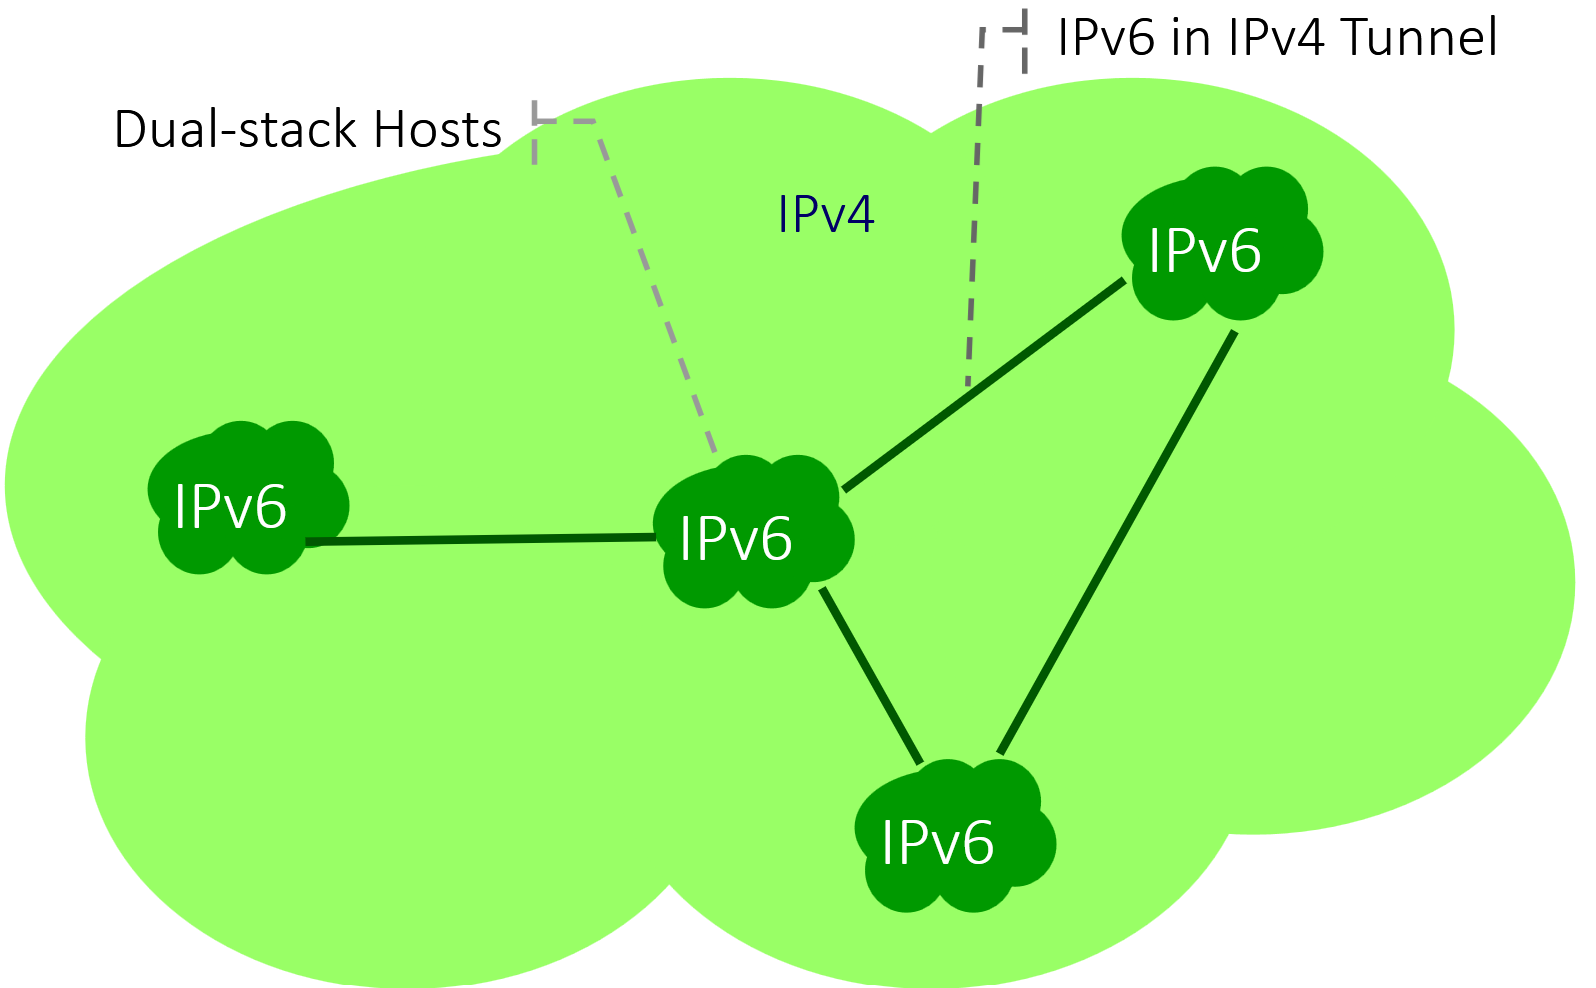
\includegraphics[width=0.5\textwidth]{capitoli/02a-IPv4-IPv6 transition/images/step1_ipv6}
\caption{Reti IPv6 isolate (Isolated IPv6 networks).}
\label{fig:fase1-transizione}
\end{figure}

\item \textbf{Crescita delle isole IPv6 (IPv6 islands grow):} Le reti IPv6 diventano più estese. Iniziano a comparire host puramente IPv6 (IPv6-only). In questa fase, diventano necessari dispositivi di traduzione (Translating Devices) posizionati ai bordi della rete per permettere la comunicazione con il mondo IPv4 esterno.

\begin{figure}[H]
\centering
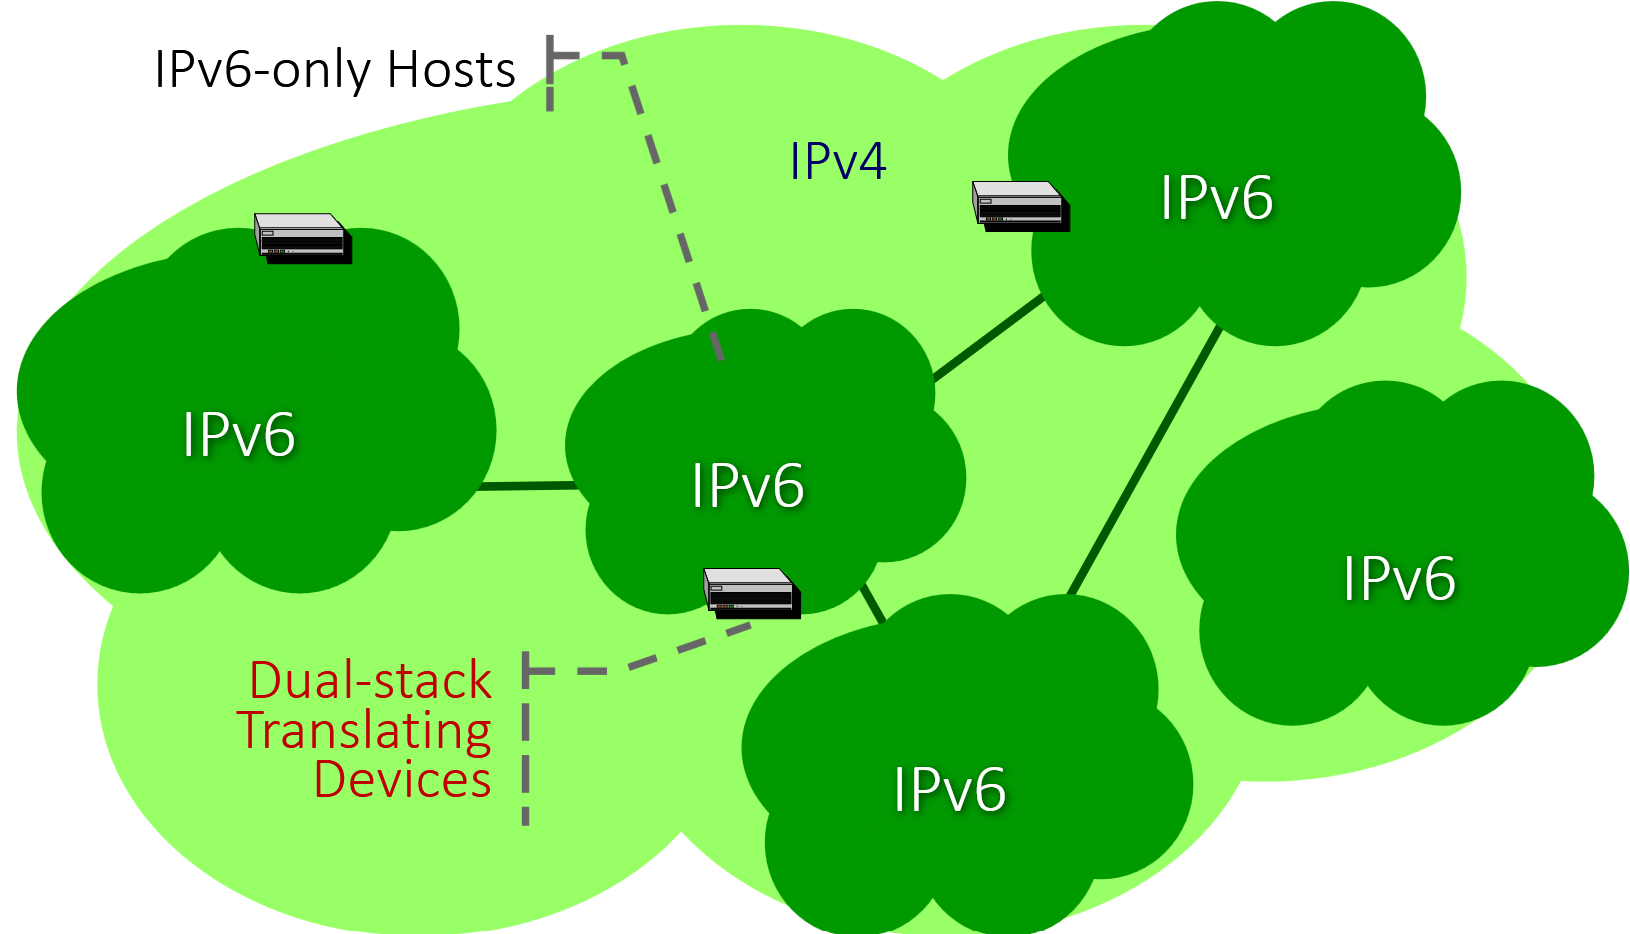
\includegraphics[width=0.5\textwidth]{capitoli/02a-IPv4-IPv6 transition/images/step2_ipv6}
\caption{Crescita delle isole IPv6 (IPv6 islands grow).}
\label{fig:fase2-transizione}
\end{figure}

\item \textbf{Connettività IPv6 nativa (Native IPv6 connectivity):} Grandi operatori (come Google, Meta, Amazon) convertono i loro data center e le loro reti in IPv6 nativo. Le isole IPv6 possono ora comunicare tra loro senza bisogno di tunnel, sfruttando la spina dorsale IPv6. I dispositivi di traduzione servono solo quando è strettamente necessario raggiungere una destinazione rimasta esclusivamente in IPv4.

\begin{figure}[H]
\centering
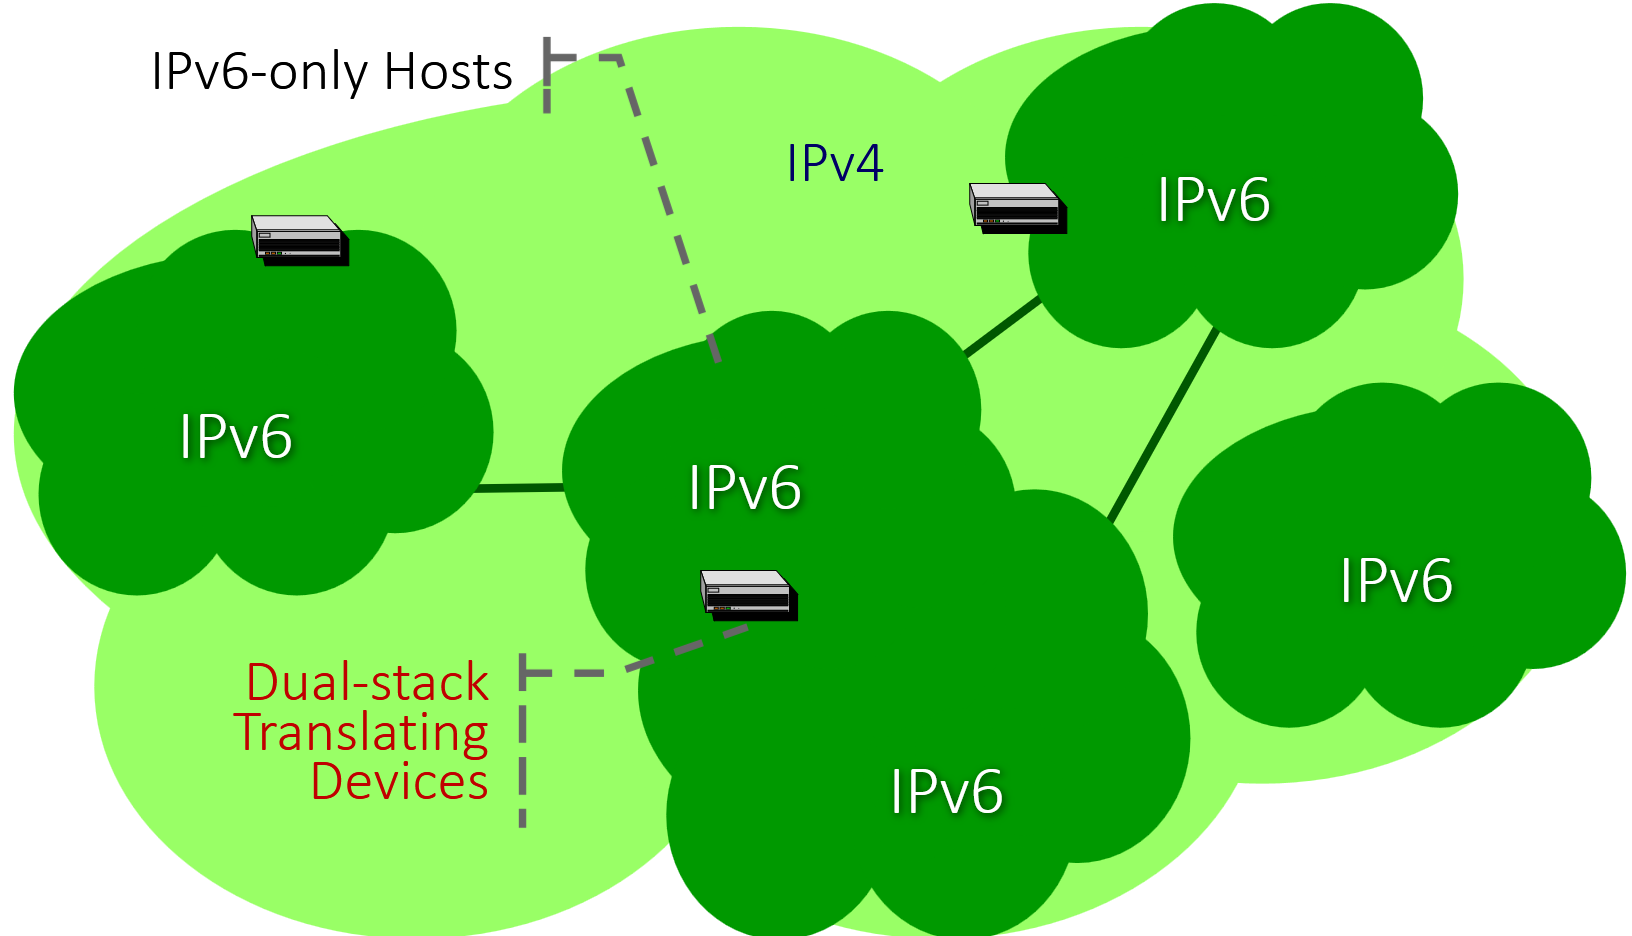
\includegraphics[width=0.5\textwidth]{capitoli/02a-IPv4-IPv6 transition/images/step3_ipv6}
\caption{Connettività IPv6 nativa tra le reti IPv6 attraverso una dorsale IPv6.}
\label{fig:fase3-transizione}
\end{figure}

\item \textbf{Subentro di IPv6 (IPv6 takes over):} Lo scenario finale. La rete globale è interamente IPv6 e i dispositivi sono IPv6-only. Qualora sopravvivano isolati dispositivi IPv4, la situazione si inverte rispetto allo step 1: sarà il traffico IPv4 a dover essere incapsulato in tunnel IPv6.

\begin{figure}[H]
\centering
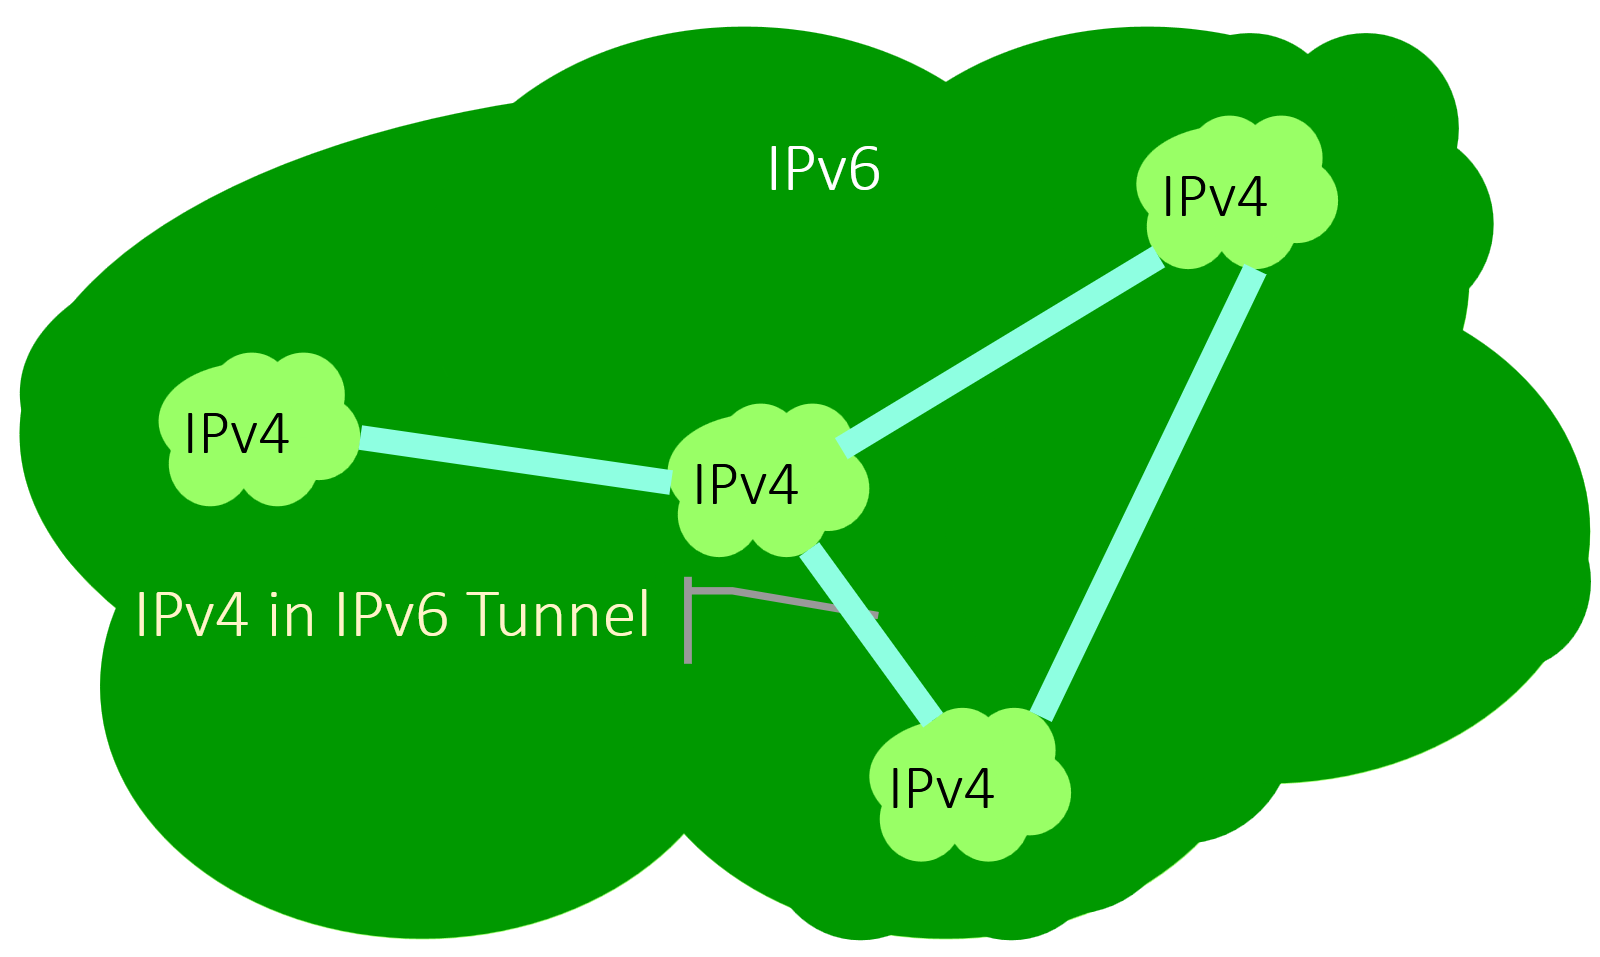
\includegraphics[width=0.5\textwidth]{capitoli/02a-IPv4-IPv6 transition/images/step4_ipv6}
\caption{Subentro di IPv6 (IPv6 takes over): la rete globale è interamente IPv6 e i dispositivi sono IPv6-only. Il traffico IPv4 viene incapsulato in tunnel IPv6 per raggiungere eventuali isole IPv4 isolate.}
\label{fig:fase4-transizione}
\end{figure}

\end{enumerate}

\subsection{Siamo pronti per lo switch-off?}
Sebbene le specifiche tecniche siano mature (la prima RFC 1883 è del 1995, divenuta Internet Standard con la RFC 8200 nel 2017), il supporto hardware e software non è più un limite. Quasi tutti i sistemi operativi moderni (Windows, Linux, macOS, Android, iOS) supportano nativamente IPv6; Apple, ad esempio, richiede dal 2016 che le app per l'App Store funzionino su reti IPv6-only. Anche i router di fascia alta gestiscono il forwarding IPv6 in hardware a \textit{line rate}.

Tuttavia, esiste ancora una vasta base installata di reti aziendali (come il Politecnico di Torino) che si affida esclusivamente a IPv4. Secondo le stime del 2026, l'adozione globale di IPv6 ha superato il 50\% (con punte del 54\% negli Stati Uniti e percentuali ancora più alte in paesi come Francia, Germania e India). Nonostante l'esistenza di obiettivi governativi (es. gli Stati Uniti puntano all'80\% di IPv6-only nei servizi federali entro il 2025; la Repubblica Ceca prevede lo spegnimento di IPv4 per il 2032), a livello globale non c'è una data condivisa. Di conseguenza, la coesistenza dei due protocolli è l'assunzione fondamentale su cui si basano le reti attuali.

\section{Approccio Dual Stack: Funzionamento e Limiti}
In una rete Dual Stack, tutti i nodi (host e router) supportano contemporaneamente IPv4 e IPv6.

\begin{figure}[H]
    \centering
    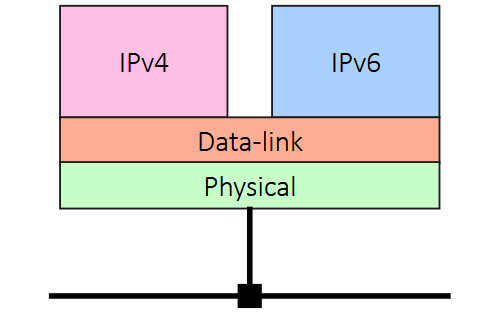
\includegraphics[width=0.3\textwidth]{capitoli/02a-IPv4-IPv6 transition/images/dual_stack}
    \caption{Esempio di rete Dual Stack: gli host e i router supportano sia IPv4 che IPv6.}
    \label{fig:dual-stack}
\end{figure}

\begin{itemize}
\item \textbf{Funzionamento:} L'host genera e riceve pacchetti IPv4 o IPv6 in base alla rete con cui sta comunicando. Tipicamente, è il Sistema Operativo dell'host a decidere quale protocollo utilizzare per instaurare una connessione, dando di norma la preferenza a IPv6 se disponibile.
\item \textbf{Svantaggi e limitazioni:} Il limite principale del Dual Stack è che \textbf{non risolve il problema dell'esaurimento degli indirizzi IPv4}. Affinché un host Dual Stack possa comunicare in IPv4, ha comunque bisogno che gli venga assegnato un indirizzo IPv4. Inoltre, questo approccio impone un onere gestionale enorme: gli amministratori di rete devono mantenere configurazioni duplicate per tutto (tabelle di routing, protocolli di routing, Access Control List, regole di firewall, sistemi di monitoraggio).
\end{itemize}
Poiché l'obiettivo finale è abbandonare IPv4, a lungo termine non è sostenibile mantenere tutti i dispositivi in Dual Stack; gli host dovranno diventare IPv6-only.

\section{Soluzioni basate su Tunneling (Fase Transitoria)}
Quando la rete di trasporto principale è IPv4, ma due reti periferiche (o host) comunicano in IPv6, si utilizza il \textit{Tunneling}.

% FIGURA ORIGINALE DA RECUPERARE DALLE SLIDE
% Slide di provenienza: 18
% Tipo: diagramma
% Descrizione: Schema di un Tunnel IPv6 over IPv4 tra due router (R1 e R2) che collegano due host (H1 e H2) su reti IPv6.
% Punto di inserimento: Qui.
% File da inserire: fig_tunneling_ipv6_ipv4
\begin{figure}[H]
\centering
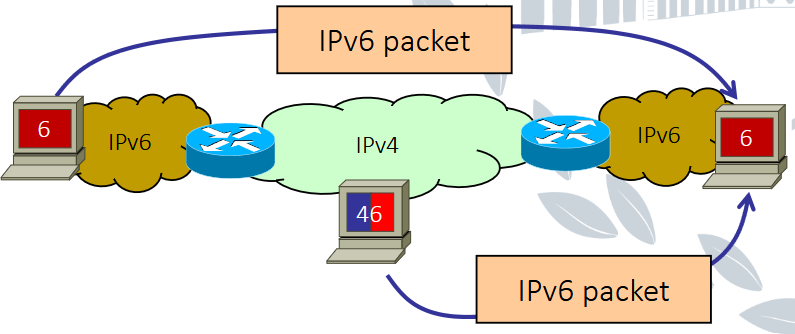
\includegraphics[width=0.5\textwidth]{capitoli/02a-IPv4-IPv6 transition/images/fig_tunneling_ipv6_ipv4}
\caption{Incapsulamento di un pacchetto IPv6 all'interno di un pacchetto IPv4 (Tunneling).}
\label{fig:tunneling}
\end{figure}

Il procedimento funziona nel modo seguente:
\begin{enumerate}
\item Un host sorgente (H1) genera un pacchetto IPv6 nativo destinato all'host ricevente (H2).
\item Il pacchetto raggiunge il router di bordo (R1), che è un router Dual Stack connesso alla rete IPv4 geografica.
\item R1 prende l'intero pacchetto IPv6 e lo inserisce come \textit{payload} all'interno di un nuovo pacchetto IPv4. L'header IPv4 esterno avrà come IP sorgente l'indirizzo IPv4 pubblico di R1 e come IP destinazione l'indirizzo IPv4 pubblico del router di bordo remoto (R2).
\item I router intermedi della rete Internet guardano solo l'header IPv4 esterno ed effettuano un normale forwarding senza sapere di trasportare traffico IPv6.
\item Il router R2 riceve il pacchetto, riconosce dal campo "Protocol" dell'header IPv4 che il payload contiene un pacchetto IPv6, estrae il pacchetto originale (decapsulamento) e lo instrada sulla propria rete locale IPv6 verso l'host H2.
\end{enumerate}

\begin{figure}[H]
    \centering
    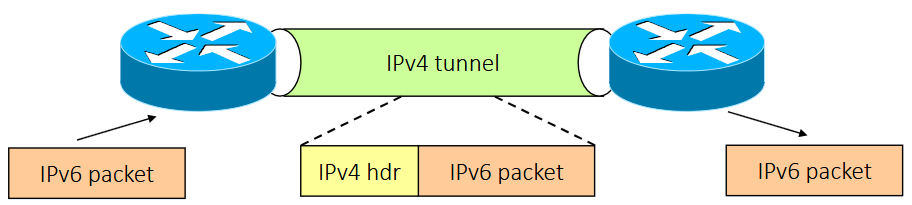
\includegraphics[width=0.5\textwidth]{capitoli/02a-IPv4-IPv6 transition/images/tunneling_ipv6_ipv4}
    \caption{Esempio di Tunnel IPv6 over IPv4 tra due router (R1 e R2) che collegano due host (H1 e H2) su reti IPv6.}
    \label{fig:tunnel-ipv6-ipv4}
\end{figure}

A livello di protocollo, questa operazione viene solitamente implementata in due modi:
\begin{itemize}
\item \textbf{Incapsulamento diretto:} L'header IPv4 indica nel campo \texttt{Protocol} il valore \texttt{41}, che segnala esplicitamente la presenza di un header IPv6 subito successivo.
\item \textbf{Utilizzo di GRE (Generic Routing Encapsulation):} Si utilizza il protocollo GRE per instaurare un canale logico tra i due router. L'header IPv4 indica GRE nel campo \texttt{Protocol}, e l'header GRE successivo specificherà che il carico utile è IPv6. Questa soluzione è preferita dagli operatori per la maggiore flessibilità e controllo sul tunnel.
\end{itemize}

\subsection{Come scoprire il Tunnel Endpoint: La soluzione storica 6to4}
La vera difficoltà del tunneling non è l'incapsulamento in sé, ma permettere a R1 di scoprire automaticamente quale sia l'indirizzo IPv4 di R2 (il \textit{tunnel endpoint}) a partire dall'indirizzo IPv6 di destinazione.

Agli albori di IPv6 era stata proposta una soluzione chiamata \textbf{6to4} (oggi deprecata). L'idea era di incorporare l'indirizzo IPv4 del router direttamente nel prefisso della rete IPv6. Ad ogni router veniva assegnato un prefisso composto fisso (\texttt{2002::/16}) seguito immediatamente dai 32 bit del suo indirizzo IPv4 pubblico.
In questo modo, quando R1 riceveva un pacchetto destinato a un indirizzo che iniziava per \texttt{2002::}, sapeva immediatamente che doveva estrarre i successivi 32 bit e usarli come indirizzo IPv4 di destinazione per la creazione del tunnel.

Questa soluzione "network-centered" era estremamente vincolante: limitava drasticamente la libertà dell'operatore nell'assegnare le subnet IPv6 e non consentiva la corretta scalabilità delle reti. Per questo motivo, meccanismi come 6to4, ISATAP e Teredo sono considerati obsoleti e non vengono più utilizzati nelle reti carrier-grade odierne.

\begin{figure}[H]
    \centering
    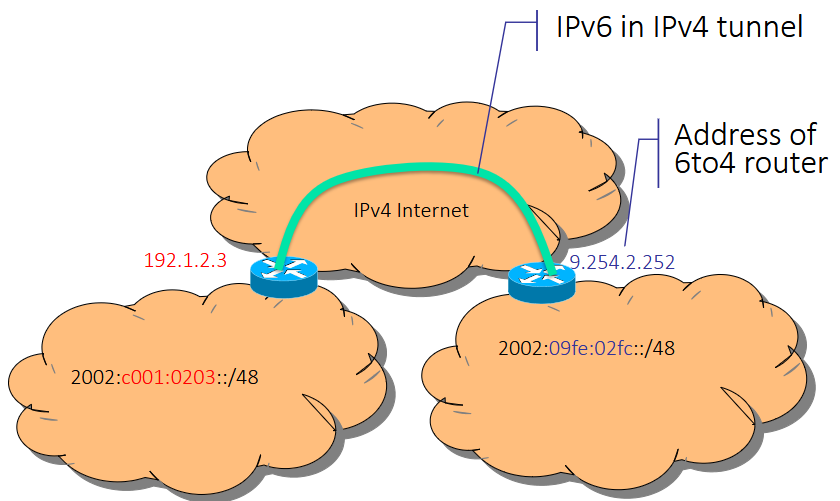
\includegraphics[width=0.5\textwidth]{capitoli/02a-IPv4-IPv6 transition/images/6to4}
    \caption{Esempio di funzionamento del tunneling 6to4, in cui l'indirizzo IPv4 del router viene incapsulato nel prefisso IPv6.}
    \label{fig:6to4}
\end{figure}

\section{Soluzioni Scalabili "Carrier-Grade"}
Gli Internet Service Provider (ISP) necessitano di soluzioni altamente scalabili, in grado di far comunicare clienti IPv6 con servizi IPv4 senza imporre vincoli sulla struttura dei prefissi.
Prima di analizzare le soluzioni per IPv6, è fondamentale comprendere come è gestito IPv4 nelle reti degli operatori oggi.

\subsection{Il ruolo fondamentale del NAT}
Attualmente, l'esaurimento degli indirizzi IPv4 obbliga l'uso intensivo del NAT (Network Address Translation).
Esistono diversi scenari di NAT:
\begin{itemize}
\item \textbf{NAT44 Domestico:} Il router di casa (CPE - Customer Premises Equipment) converte gli indirizzi privati (es. \texttt{192.168.0.0/24}) dei dispositivi locali in un unico indirizzo pubblico assegnato dall'operatore.
\item \textbf{Carrier Grade NAT (CGN) / Large Scale NAT (LSN):} Gli operatori (sia per reti fisse che cellulari) non hanno più sufficienti indirizzi IPv4 pubblici da dare a ogni singolo modem. Assegnano pertanto al CPE un indirizzo \textit{Provider Private} (es. dallo spazio condiviso \texttt{100.64.0.0/10}, RFC 6598) e posizionano un gigantesco NAT all'interno della propria rete (il CGN) per tradurre il traffico di migliaia di utenti prima di immetterlo su Internet.
\item \textbf{Doppio NAT:} Una combinazione dei due (frequente in operatori come Fastweb). Il traffico subisce un primo NAT in casa (sul CPE) e un secondo NAT a livello di operatore (sul CGN).
\end{itemize}

\begin{figure}[H]
    \centering
    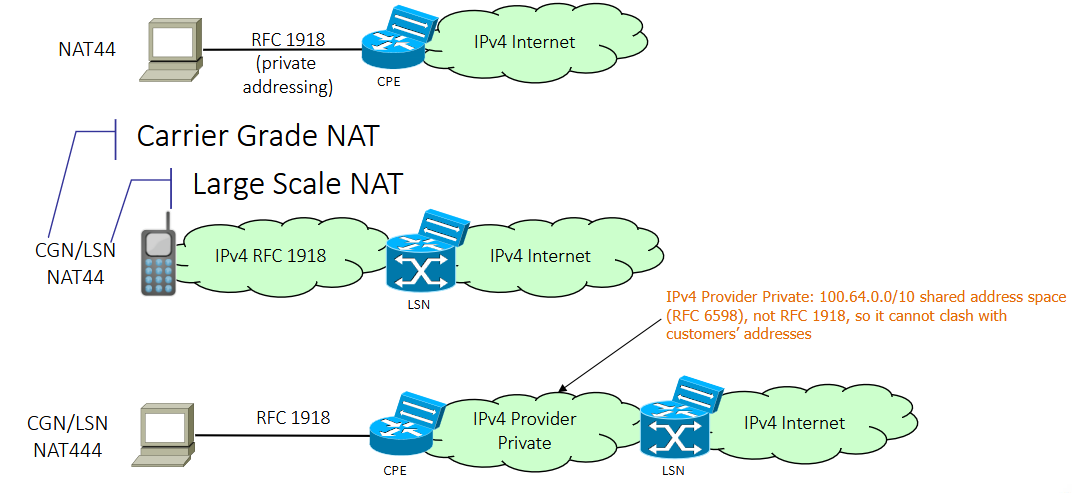
\includegraphics[width=0.7\textwidth]{capitoli/02a-IPv4-IPv6 transition/images/nat}
    \caption{Rappresentazione dei tre scenari di NAT descritti: NAT44 domestico, Carrier Grade NAT (CGN) e doppio NAT.}
    \label{fig:nat}
\end{figure}

Il NAT è un male necessario: crea problemi per le connessioni in ingresso (i server dietro NAT non sono direttamente raggiungibili senza complessi \textit{port forwarding}), rappresenta un collo di bottiglia e un Single Point of Failure (SPOF) critico per la rete dell'operatore.
Le tecnologie di transizione IPv6 devono tenere conto di questi problemi e cercano di gestirli attraverso l'introduzione di un apparato chiave nella rete dell'operatore: l'\textbf{AFTR (Address Family Transition Router)}, che funge da concentratore di tunnel o da dispositivo di traduzione.

% FIGURA ORIGINALE DA RECUPERARE DALLE SLIDE
% Slide di provenienza: 28-29
% Tipo: schema logico
% Descrizione: Rappresentazione dell'architettura con CPE (lato utente) e AFTR (lato provider) in contesti IPv6.
% Punto di inserimento: Qui.
% File da inserire: fig_cpe_aftr_architecture
\begin{figure}[H]
\centering
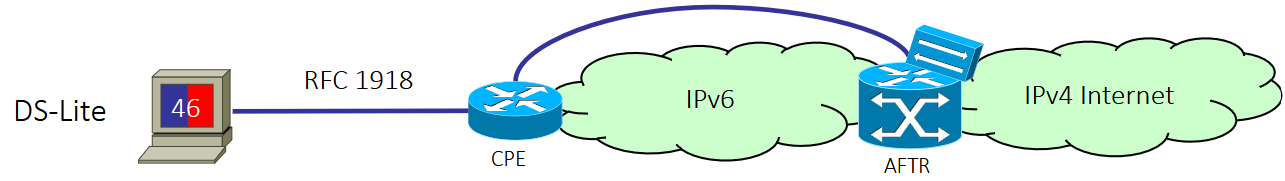
\includegraphics[width=0.85\textwidth]{capitoli/02a-IPv4-IPv6 transition/images/cpe_aftr_architecture}
\caption{Architettura tipica con Customer Premises Equipment (CPE) e Address Family Transition Router (AFTR).}
\label{fig:cpe-aftr}
\end{figure}

\subsection{DS-Lite (Dual-Stack Lite)}
DS-Lite è una soluzione in cui la rete dell'operatore (backbone) è puramente IPv6, ma l'utente a casa necessita ancora di connettività IPv4 (Dual-Stack all'edge).

\textbf{Meccanismo:}
\begin{enumerate}
\item L'host invia un normale pacchetto IPv4 con un indirizzo sorgente privato.
\item Il CPE (detto \textit{B4} in questa specifica) incapsula il pacchetto IPv4 in un tunnel IPv6, senza eseguire alcuna operazione di NAT locale.
\item Il pacchetto tunnelato viaggia sulla rete IPv6 dell'operatore fino all'AFTR (che agisce come Carrier Grade NAT).
\item L'AFTR decapsula il tunnel, estrae il pacchetto IPv4 privato e \textbf{svolge il NAT44}, sostituendo l'IP privato con il proprio IP pubblico e assegnando una porta.
\end{enumerate}

\begin{figure}[H]
    \centering
    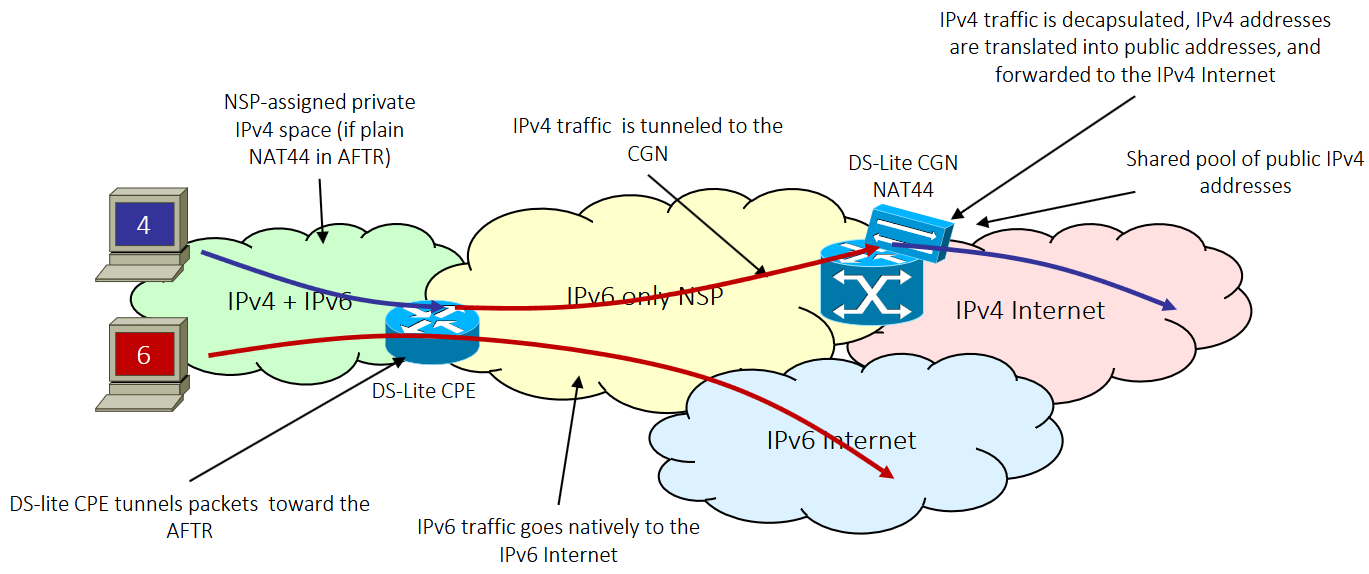
\includegraphics[width=0.85\textwidth]{capitoli/02a-IPv4-IPv6 transition/images/dslite}
    \caption{Funzionamento di DS-Lite: il CPE incapsula i pacchetti IPv4 in tunnel IPv6 verso l'AFTR, che esegue il NAT44.} 
    \label{fig:ds-lite}
\end{figure}

\textbf{Svantaggi e criticità:}
Il vero problema di DS-Lite risiede nella gestione delle risposte di ritorno e nella memoria richiesta sull'AFTR. In un NAT tradizionale, la tabella di stato associa l'IP privato e la porta sorgente all'IP pubblico e alla porta convertita.
In DS-Lite, poiché lo stesso IP privato (es. \texttt{192.168.0.10}) può essere utilizzato da migliaia di CPE differenti connessi allo stesso AFTR, l'AFTR deve obbligatoriamente salvarsi \textbf{anche l'indirizzo IPv6 del CPE} all'interno della sua tabella NAT.
Quando l'AFTR riceve il pacchetto di risposta da Internet, deve:
\begin{itemize}
\item Individuare a quale flusso appartiene tramite la porta di destinazione.
\item Tradurre l'indirizzo IP pubblico nell'indirizzo IP privato originale dell'host.
\item Recuperare dalla tabella l'indirizzo IPv6 del CPE per poter ricostruire il tunnel IPv6 a ritroso.
\end{itemize}
Questo richiede il mantenimento di uno stato "per flusso" (\textit{stateful}) enorme. La tabella delle connessioni esplode di dimensioni. Inoltre, il NAT è interamente sotto il controllo dell'operatore, impedendo all'utente di configurare il \textit{port forwarding}.

\subsection{A+P (Address plus Port)}
Per alleviare il carico computazionale e di memoria sull'AFTR generato dal DS-Lite, è stata sviluppata l'architettura A+P (Address plus Port).

L'idea innovativa è riportare l'operazione di NAT44 sotto il controllo del CPE dell'utente finale, mitigando al contempo la scarsità di indirizzi pubblici. L'operatore assegna ai CPE un indirizzo IPv4 pubblico, ma poiché non ci sono abbastanza indirizzi per tutti, \textbf{lo stesso indirizzo IPv4 pubblico viene condiviso tra più CPE}.

Per differenziarli, l'operatore assegna a ciascun CPE un \textbf{range specifico di porte TCP/UDP} (ad esempio, al CPE 1 le porte da 6000 a 6010, al CPE 2 le porte da 6011 a 6020).
\begin{itemize}
\item Il CPE esegue il NAT e maschera tutto il traffico locale sfruttando unicamente il blocco di porte che gli è stato assegnato.
\item L'assegnazione delle porte può essere statica o negoziata dinamicamente tramite protocolli come il PCP (Port Control Protocol) o DHCPv6.
\item L'AFTR diventa un semplice terminatore di tunnel. Non deve più mantenere una mastodontica tabella NAT per ogni singolo flusso; gli basta mantenere un mapping statico o semi-statico che associa un indirizzo IPv4 e un determinato range di porte al rispettivo indirizzo IPv6 del CPE.
\end{itemize}
In questo modo, quando riceve un pacchetto in ritorno da Internet, l'AFTR osserva l'indirizzo IPv4 e la porta, capisce immediatamente a quale CPE appartiene la risposta e costruisce il tunnel IPv6 corretto.

\begin{figure}[H]
    \centering
    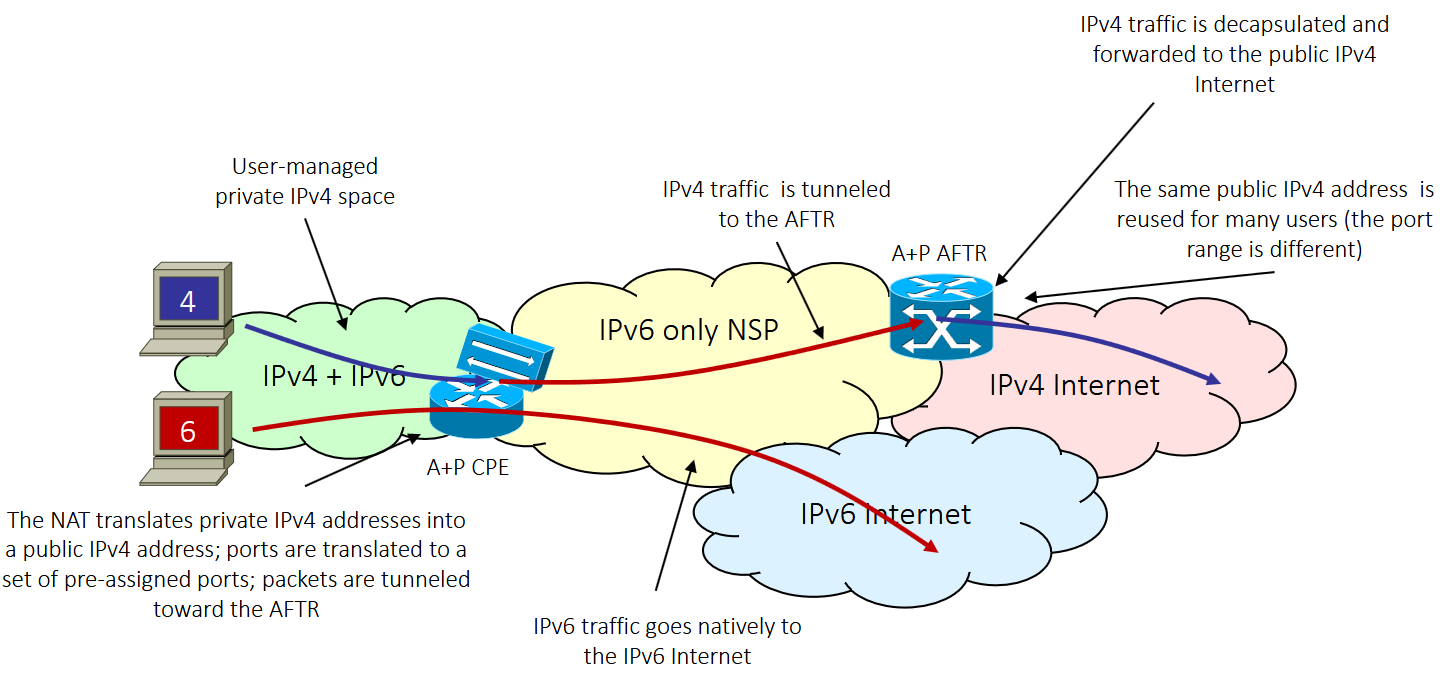
\includegraphics[width=0.85\textwidth]{capitoli/02a-IPv4-IPv6 transition/images/a-p}
    \caption{Funzionamento di A+P: il CPE esegue il NAT e maschera il traffico locale, mentre l'AFTR si occupa solo del terminatore di tunnel.}
    \label{fig:a-p}
\end{figure}

\subsection{MAP-E e MAP-T (Stateless A+P)}
L'evoluzione diretta di A+P si chiama MAP (Mapping of Address and Port) ed è la soluzione impiegata attualmente nei moderni provider (molto diffusa ad esempio in Giappone).

L'obiettivo di MAP è rendere l'AFTR (chiamato qui \textit{Border Relay}) completamente \textbf{stateless}: non deve mantenere alcuna tabella in memoria, né per i flussi né per l'associazione CPE-porte.
Per ottenere questo risultato, l'algoritmo \textbf{scrive l'informazione di routing direttamente all'interno dell'indirizzo IPv6}. Il prefisso IPv6 assegnato al CPE viene generato incastonando matematicamente al suo interno l'indirizzo IPv4 pubblico condiviso e l'identificativo del set di porte (PSID).

In questo modo, quando il traffico di ritorno attraversa il Border Relay, questo dispositivo può derivare istantaneamente l'indirizzo IPv6 del CPE destinazione estraendolo direttamente dai bit dell'indirizzo e della porta IPv4 del pacchetto in arrivo, senza dover consultare alcuna tabella.

Esistono due varianti:
\begin{itemize}
\item \textbf{MAP-E (Encapsulation):} Come in DS-Lite, il pacchetto IPv4 è incapsulato (\textit{tunneled}) dentro un header IPv6.
\item \textbf{MAP-T (Translation):} Non si fa tunneling. L'header IPv4 viene letteralmente scartato e tradotto (\textit{header translation}) in un header IPv6, la cui destinazione viene calcolata dinamicamente per veicolare l'informazione originale.
\end{itemize}

\section{Connettività da host IPv6-only verso server IPv4}
Fino a questo punto abbiamo trattato il trasporto di traffico IPv4 su dorsali IPv6. L'ultimo scenario da considerare --- che diventerà presto la norma --- è quello in cui l'operatore dismette completamente IPv4 anche presso l'utente finale: l'host domestico riceve solo un indirizzo IPv6 (\textbf{IPv6-only host}).
Tuttavia, parte di Internet globale (vecchi server, servizi legacy) è ancora esclusivamente IPv4. Come può l'utente IPv6-only raggiungere un web server IPv4-only?

\subsection{NAT64 e DNS64}
La combinazione di NAT64 e DNS64 è un'elegante soluzione ingegneristica per risolvere questo problema. Il suo funzionamento si basa sull'interazione fondamentale del protocollo DNS.

% FIGURA ORIGINALE DA RECUPERARE DALLE SLIDE
% Slide di provenienza: 37-39
% Tipo: schema di funzionamento
% Descrizione: Flusso di risoluzione nomi e forwarding di pacchetti con DNS64 e NAT64, inclusa la sintesi del record AAAA.
% Punto di inserimento: Qui.
% File da inserire: fig_nat64_dns64
\begin{figure}[H]
\centering
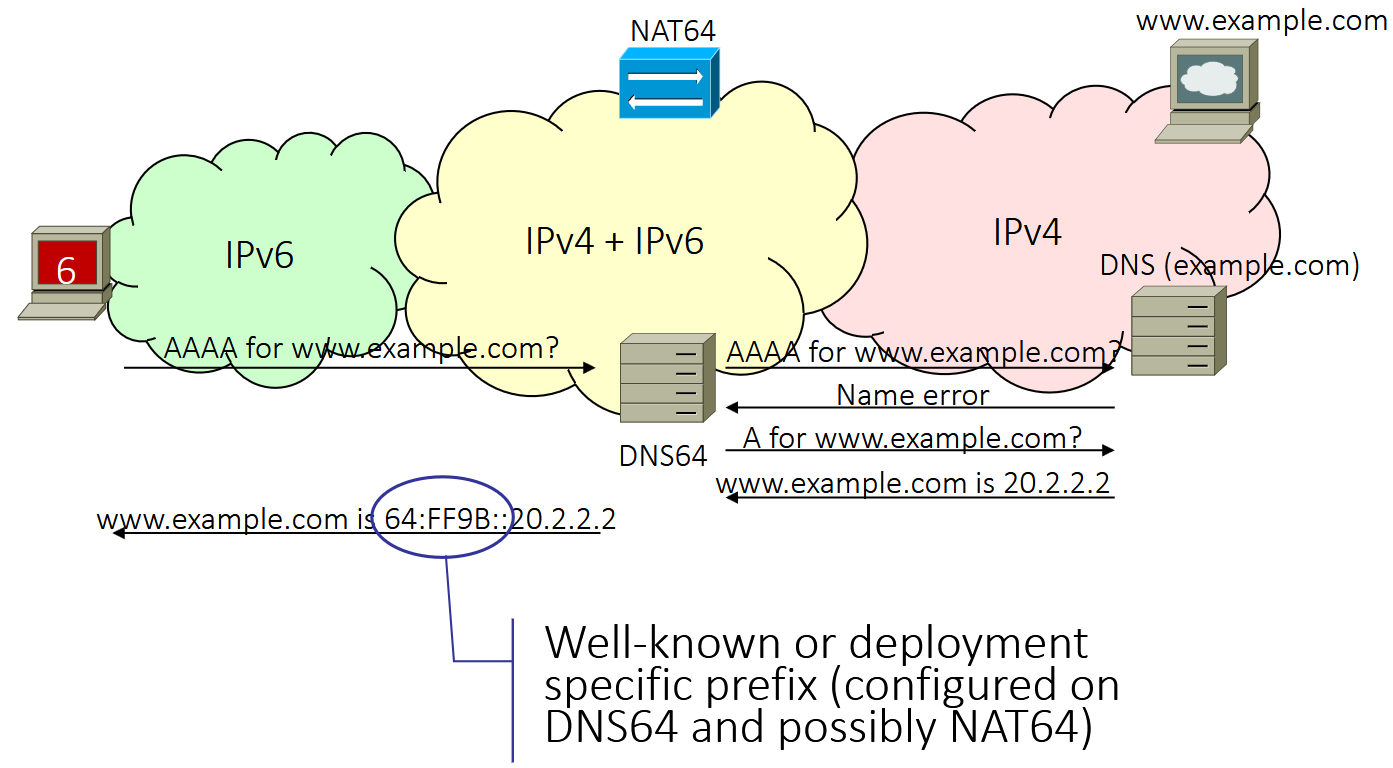
\includegraphics[width=0.65\textwidth]{capitoli/02a-IPv4-IPv6 transition/images/dns64}
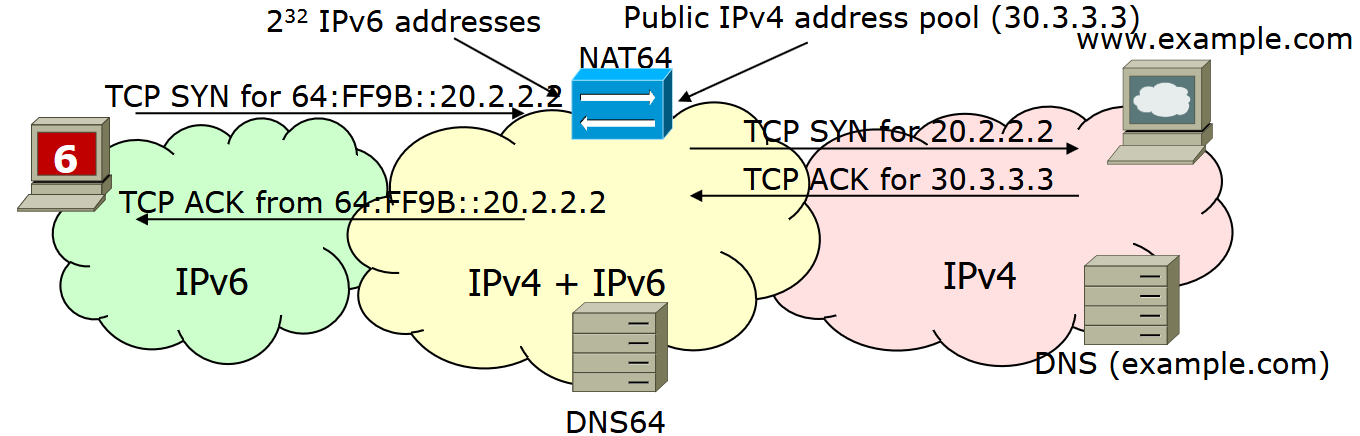
\includegraphics[width=0.65\textwidth]{capitoli/02a-IPv4-IPv6 transition/images/nat64}
\caption{Funzionamento congiunto di DNS64 e NAT64 per permettere a host IPv6 di contattare servizi IPv4.}
\label{fig:nat64-dns64}
\end{figure}

\textbf{Funzionamento:}
\begin{enumerate}
\item L'host IPv6-only vuole contattare un dominio (es. \texttt{example.com}). Trattandosi di un host IPv6, richiede al proprio server DNS locale un record di tipo AAAA.
\item Questo server DNS locale è un dispositivo speciale, il \textbf{DNS64}. Esso contatta il server autoritativo globale per ottenere il record AAAA.
\item Il server autoritativo risponde che il dominio possiede solo un record A (indirizzo IPv4, es. \texttt{2.2.2.2}).
\item A questo punto il DNS64 interviene: invece di restituire un errore all'host, "manipola" la risposta e \textbf{sintetizza un indirizzo IPv6 fasullo}. Prende l'indirizzo IPv4 ricevuto, lo accoda a un prefisso IPv6 speciale dedicato (spesso il prefisso well-known \texttt{64:ff9b::/96} oppure uno definito dall'operatore) e restituisce questa finta risposta AAAA all'host (es. \texttt{64:ff9b::2.2.2.2}).
\item L'host crede di avere a che fare con un server IPv6 e inizia la connessione TCP (inviando il SYN) verso l'indirizzo finto.
\item Il routing dell'operatore è configurato affinché tutto il traffico destinato a quel prefisso speciale finisca a un router traduttore, il \textbf{NAT64}.
\item Il NAT64 (lavorando in modalità \textit{stateful} out-bound) estrae gli ultimi 32 bit dall'IP destinazione fasullo per recuperare il vero IP IPv4 del server (\texttt{2.2.2.2}). Sostituisce l'IP sorgente IPv6 dell'utente con un indirizzo IP IPv4 pubblico proveniente dal proprio pool di indirizzi, salvando questa corrispondenza nella sua tabella di stato NAT.
\item Traduce l'header da IPv6 a IPv4 e invia il pacchetto. Il server riceve il traffico come se provenisse dal NAT64, vi risponde in IPv4, e il NAT64 esegue il processo inverso per recapitare il pacchetto IPv6 all'host.
\end{enumerate}

\textbf{Limitazioni critiche del NAT64/DNS64:}
Questa architettura, per quanto fluida, presenta due forti limitazioni:
\begin{itemize}
\item \textbf{Richiede obbligatoriamente l'uso di nomi a dominio:} Se un utente (o un'applicazione legacy, come una vecchia telecamera IP o un videogioco) tenta di collegarsi specificando esplicitamente un indirizzo IPv4 numerico (es. il comando \texttt{ping 1.2.3.4} oppure digitando l'IP nel browser), il processo fallisce. Il DNS non viene interpellato, l'indirizzo fasullo non viene generato e l'host IPv6-only non ha modo di instradare un pacchetto verso una destinazione 32-bit.
\item \textbf{Incompatibilità con DNSSEC:} Il protocollo DNSSEC garantisce, tramite firme crittografiche, che le risposte del DNS non subiscano alterazioni o manipolazioni durante il tragitto. Poiché il DNS64 intercetta la risposta A autentica e sintetizza artificialmente un record AAAA, un client che valuta le firme crittografiche (DNSSEC validating client) classificherebbe questa risposta come una manomissione e respingerebbe la connessione.
\end{itemize}

\subsection{464XLAT e Accesso IPv6-only}
Per superare i gravi limiti imposti dal NAT64/DNS64 (particolarmente castranti per le reti mobili e le app per smartphone), è stata introdotta la soluzione \textbf{464XLAT}.

Questa tecnologia risolve l'incompatibilità con applicazioni che utilizzano indirizzi IPv4 letterali suddividendo l'architettura in due componenti traduttori:
\begin{enumerate}
\item \textbf{CLAT (Customer-side Translator):} È un piccolo programma, demone o modulo del sistema operativo che gira localmente sull'host dell'utente (ad esempio, sul sistema Android o sul CPE di casa). Quando un'applicazione tenta di aprire una connessione diretta a un indirizzo numerico IPv4, il CLAT la intercetta localmente. Esegue una traduzione \textit{stateless} (SIIT), convertendo il pacchetto in un formato IPv6 destinato al famoso prefisso speciale \texttt{64:ff9b::/96}.
\item \textbf{PLAT (Provider-side Translator):} Non è altro che il router NAT64 standard posizionato nella rete dell'operatore. Il PLAT riceve il pacchetto IPv6 dal CLAT e lo converte normalmente in IPv4 per recapitarlo a destinazione.
\end{enumerate}

% FIGURA ORIGINALE DA RECUPERARE DALLE SLIDE
% Slide di provenienza: 41
% Tipo: schema logico
% Descrizione: Architettura del 464XLAT con l'interazione tra l'host con il programma CLAT, il router PLAT (NAT64) e le rispettive traduzioni.
% Punto di inserimento: Qui.
% File da inserire: fig_464xlat_architecture
\begin{figure}[H]
\centering
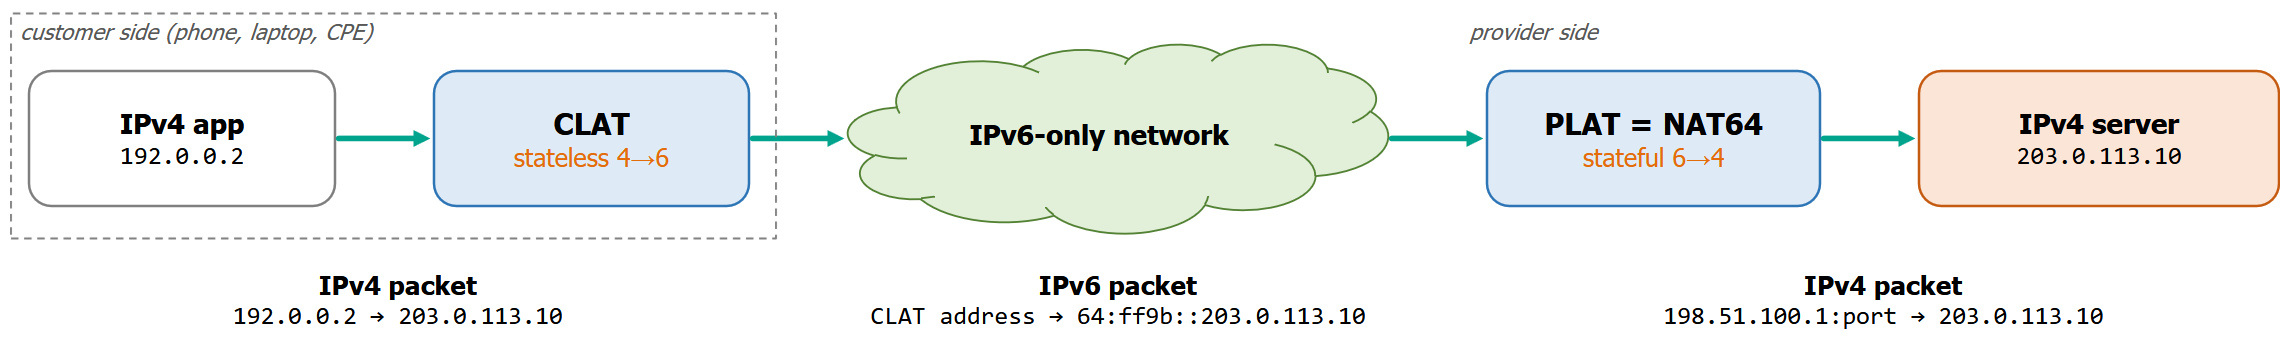
\includegraphics[width=0.85\textwidth]{capitoli/02a-IPv4-IPv6 transition/images/464xlat_architecture}
\caption{Architettura 464XLAT, che abilita il traffico IPv4 trasparente su infrastrutture puramente IPv6 grazie a CLAT e PLAT.}
\label{fig:464xlat}
\end{figure}

Il vantaggio di 464XLAT risiede nel fatto che le applicazioni sul dispositivo "credono" di disporre di una connessione IPv4 attiva. Il sistema inganna le applicazioni gestendo la traduzione direttamente nel dispositivo finale (CLAT) prima ancora che il traffico imbocchi la rete dell'operatore.
Affinché questo modello funzioni, tutti i router della rete IPv6 e il CLAT stesso devono conoscere la rotta (routing table) per raggiungere il prefisso \texttt{64:ff9b::/96}, permettendo spesso al PLAT di essere distribuito in \textit{Anycast} per garantire affidabilità e bilanciamento del carico.